\chapter[MATERIAIS E MÉTODOS]{MATERIAIS E MÉTODOS}

Neste capítulo apresentam-se os métodos empregados na proposta deste trabalho. Um processo de classificação, conforme ilustrado na Figura \ref{fig:4}, pode ser dividido em seis etapas \cite{kadhim2019survey}: coleta de dados, pré-processamento, extração de características, redução de dimensionalidade, aplicação da técnica de classificação e avaliação de desempenho.

\begin{figure}[H]
    \centering
    \caption{Etapas do processo de classificação}. 
    \label{fig:4}
 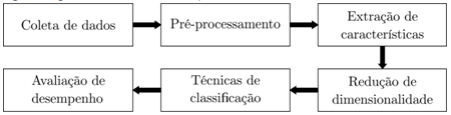
\includegraphics[width=120mm]{images/fig6.png}
    \fonte{Adaptado de \cite{kadhim2019survey}.}
\end{figure}

%% INICIO DESCRIÇÃO BASE DE DADOS
\section{BASES DE DADOS}
A base de dados utilizada 3W dataset (VARGAS et al., 2019) é pública e contém 1.984
instâncias de séries temporais da produção de poços de petróleo marítimos do tipo surgente
(poços que conseguem escoar os fluidos produzidos até a plataforma com sua própria
pressão). Essas instâncias foram separadas em: operação em condições normais e anomalias.
As anomalias foram organizadas em oito classes. Essa base pode ser utilizada tanto para
detecção quanto para classificação de anomalias em poços de petróleo.


%% INICIO PRÉ-PROCESSAMENTO
\section{PRÉ-PROCESSAMENTO}
A etapa de pré-processamento trata da preparação inicial do conjunto de dados coletado. No
caso de séries temporais, nessa etapa, inclui-se a análise dos dados, geração de gráficos para
entendimento do dados, remoção de valores nulos e/ou congelados e re-amostragens de
observações das séries temporais para balanceamento da base de dados.

%% INICIO PRÉ-PROCESSAMENTO
\section{EXTRAÇÃO DE CARACTERÍSTICAS }
A partir de cada amostra de série temporal, foram extraídas e utilizadas como características a
mediana, média, desvio padrão, variância, máximo e mínimo para cada variável. Para esta
extração de características das séries temporais foi utilizada a biblioteca tsfresh2
(Time seriesfeature extraction) (CHRIST et al., 2018) na configuração de parâmetros mínimos, de forma a
ser possível reproduzir os resultados iniciais gerados por Vargas (2019).

\begin{figure}[H]
    \centering
    \caption{Descrição das variáveis das séries temporais presentes no 3W dataset}. 
    \label{fig:10}
 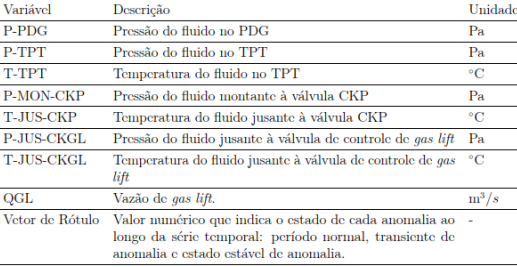
\includegraphics[width=120mm]{images/fig10.png}
    \fonte{\cite{vargas2019base}}
\end{figure}


%% INICIO REDUÇÃO DE DIMENSIONALIDADE
\section{REDUÇÃO DE DIMENSIONALIDADE}
Após a extração de características, é possível que se tenha uma grande quantidade de
características, e pode ser necessário reduzir os custos de processamento. Esse processo é
denominado de redução de dimensionalidade.Foram utilizadas as seguintes tecnicas:

\subsection{KERNEL PRINCIPAL COMPONENT ANALYSIS (KPCA)}
\subsection{ISOMETRIC MAPPING (ISOMAP)}
\subsection{DEEP MANIFOLD TRANSFORMATION(DMT)}


%% INICIO TÉCNICAS DE CLASSIFICAÇÃO
\section{TÉCNICAS DE CLASSIFICAÇÃO}

%% INICIO AVALIAÇÃO DE DESEMPENHO
\section{AVALIAÇÃO DE DESEMPENHO}
Na última etapa do processo de classificação, é necessário avaliar o desempenho obtido. De
acordo com Kowsari et al. (2019), essa avaliação é geralmente feita por meio de métricas, tais
como acurácia, revogação, precisão ou por meio do indicador medida-F1. Estas métricas são
obtidas a partir da matriz de confusão, ilustrada na Tabela 4, na qual são listados os valores
verdadeiros positivos (ou True Positive - TP), falsos positivos (ou False Positive FP),
verdadeiros negativos (ou True Negative - TN) e falsos negativos (ou False Negative - FN)
para cada classe.
Nesse trabalho, foi utilizada a métrica de medida F1 para análise de desempenho. Os testes
estatísticos de Friedman e Wilcoxon também foram aplicados aos resultados dos
experimentos de forma a permitir comparações entre os classificadores entre si e com os
resultados do trabalho de Vargas (2019).
%%% INICIO PARTE REVISÃO
\todo[inline]{FIM -  APENAS TEXTO BASE }